\documentclass{classrep}
\usepackage[utf8]{inputenc}
\frenchspacing

\usepackage{graphicx}
\usepackage[usenames,dvipsnames]{color}
\usepackage[hidelinks]{hyperref}
\usepackage{float}
\usepackage{setspace}
\usepackage{amsmath, amssymb, mathtools}

\usepackage{booktabs}
\usepackage{graphicx}
\usepackage{pdflscape}

\setlength{\abovecaptionskip}{-10pt}

\studycycle{Informatyka stosowana, studia dzienne, II st.}
\coursesemester{II}
\coursename{Analiza danych złożonych}
\courseyear{2020/2021}

\courseteacher{dr hab. inż. Agnieszka Duraj}
\coursegroup{poniedziałek, 11:45}

\author{%
  \studentinfo{Paweł Galewicz}{234053}\\
  \studentinfo{Karol Podlewski}{234106}%
}

\title{Etap 1: Badanie zmienności trendu\\w strumieniu danych}

\begin{document}
\maketitle

\setstretch{1.5}

\tableofcontents
\setstretch{1.25}
\newpage

\section{Cel}

Zadanie polegało na analizie strumienia danych jego charakterystyki pod kątem pojawiania się w nich zmian – tzw. Detekcja Dryftu, Concept drift.

\section{Implementacja}

Program został stworzony w języku Python w wersji 3.8.6, przy wsparciu bibliotek scikit-multiflow oraz scikit w celu skorzystania z algorytmów przeznaczonych do detekcji dryftu oraz klasyfikacji.

Wybranym przez nas klasyfikatorem był algorytm K najbliższych sąsiadów. Do detekcji dryftów wykorzystaliśmy algorytmy DDM, EDDM, ADWIN oraz Page-Hinkley.

Wykorzystano też bibliotekę argparse - w stworzonym rozwiązaniu w łatwy sposób można określić większość parametrów algorytmów, takich jak liczbę sąsiadów w KNN czy deltę w ADWIN, a także podział zbioru treningowego oraz sam plik z danymi.

\section{Opis algorytmów}

Wykorzystane w programie algorytmy działają w następujące sposoby.

\subsection{DDM}

Algorytm Drift Detection Method opiera się na założeniu, że wraz z wzrostem liczby obserwacji liczba błędów powinna maleć, bądź być na tym samym poziomie. Dla modelu wyliczana jest minimalna stopa błędu, określana dwoma czynnikami: $p_{min}$ i $s_{min}$. Na postawie tych czynników wyznaczane są progi ostrzegawcze i alarmowe, które następnie oblicza się dla i-tego punktu wzorem:
\begin{align*}
    p_i + s_i \geq p_{min} + \alpha * s_{min}\\
    p_i + s_i \geq p_{min} + \beta * s_{min}
\end{align*}

Przekroczenie progu alarmowego może świadczyć o wystąpieniu dryftu.

\subsection{EDDM}

Early Drift Detection Method jest modyfikacją DDM, w której progi detekcji opierają się na odległościach między kolejnymi błędami. Dzięki temu podejściu, algorytm jest w stanie wykryć pojawienie się stopniowych zmian w modelu, z czym DDM nie potrafił sobie poradzić. Progi wyliczane są wzorami:

\begin{align*}
    \frac{p^`_i + 2 * s^`_i}{p^`_{max} + 2 * s^`_{max}} < \alpha \\ \\
    \frac{p^`_i + 3 * s^`_i}{p^`_{max} + 3 * s^`_{max}} < \beta
\end{align*}

\subsection{ADWIN}

Algorytm ADWIN (ADaptive WINdowing) to algorytm opierający się dynamicznym dostosowaniu rozmiaru okna czasowego - podobnie jak algorytm FLORA2 \cite{AdwinFlora}. Jedynym parametrem, który musi zostać określony przed przebiegiem algorytmu jest $\delta \epsilon (0, 1)$, która określa wrażliwość algorytmu na detekcję dryftu.

ADWIN, analizując kolejne obserwacje, dodaje je do okna czasowego, następnie sprawdza okno w celu wyłapania dryftu - w tym celu porównuje dwa odpowiednio duże okna. Dryft jest wykryty, kiedy wartości między oknami odpowiednio mocno się różnią. Algorytm rozszerza okno tak długo, jak nie wykryje żadnego dryftu - kiedy to zrobi, zmniejsza okno poprzez wyrzucenie starszych wartości \cite{Adwin}. 

\subsection{Page-Hinkley}

Page-Hinkley to algorytm, który opiera się na obliczaniu średniej z dotychczasowych wartości przekazanych ze strumienia danych. Algorytm bazuje na teście statystycznym Page-Hinkley \cite{Page}. Przyjmowany jest pewien dopuszczalny próg nagłej zmiany średniej wartości ze strumienia. Przyjmowaną hipotezą jest brak zmian, do której na bieżąco wykonywane są dwa testy, które mają za zadanie określić, czy wystąpił istotny wzrost bądź spadek. Osiągnięcie go zaprzecza przyjętej hipotezie - w przypadku Concept Drift,  świadczy to o wystąpieniu istotnej zmiany w strumieniu. 

\section{Badania}

Celem przeprowadzonych przez nas badań było sprawdzenie możliwości detekcji zmian dryftu dla kolejnych algorytmów na zadanym strumieniu danych. W tym celu stworzyliśmy model klasyfikatora z wykorzystaniem wykorzystując algorytm K najbliższych sąsiadów. Liczba sąsiadów w algorytmie KNN była na stałe ustawiona na 5, a zbiór treningowy stanowił 20\% wszystkich danych. Dla wyuczonego modelu wygenerowaliśmy statystyki dokładności. 

Następnym etapem badań było testowanie kolejnych próbek zestawu testowego, które miały symulować nowe dane przychodzące ze strumienia danych. Otrzymane predykcje każdej nowej próbki wysyłane były do poszczególnych algorytmów. Algorytmy te monitorowały liczby błędnych predykcji -- na tej podstawie określały, czy wystąpiły istotne zmiany w modelu danych przychodzącym z symulowanego strumienia. W takim przypadku zapisywany zostawał indeks danej próbki. 

Po uzyskaniu listy indeksów próbek, przy których dany algorytm stwierdzał zmianę dryftu, nanieśliśmy je na wykres zmian dokładności klasyfikatora.

Wybrany przez nas zbiór danych to \href{https://www.kaggle.com/jsphyg/weather-dataset-rattle-package}{\textbf{Rain in Australia}}, który zawiera historię danych pogodowych z 10 lat (data, lokalizacja, temperatury, opady, wiatr, ciśnienie, wilgotność, nasłonecznienie itp) wraz z informacją czy następnego dnia padało - jest to cel klasyfikacji dla tego zbioru danych.\\

Z badań otrzymaliśmy następujące wyniki.

\subsection{DDM}

\begin{figure}[H]
    \centering
    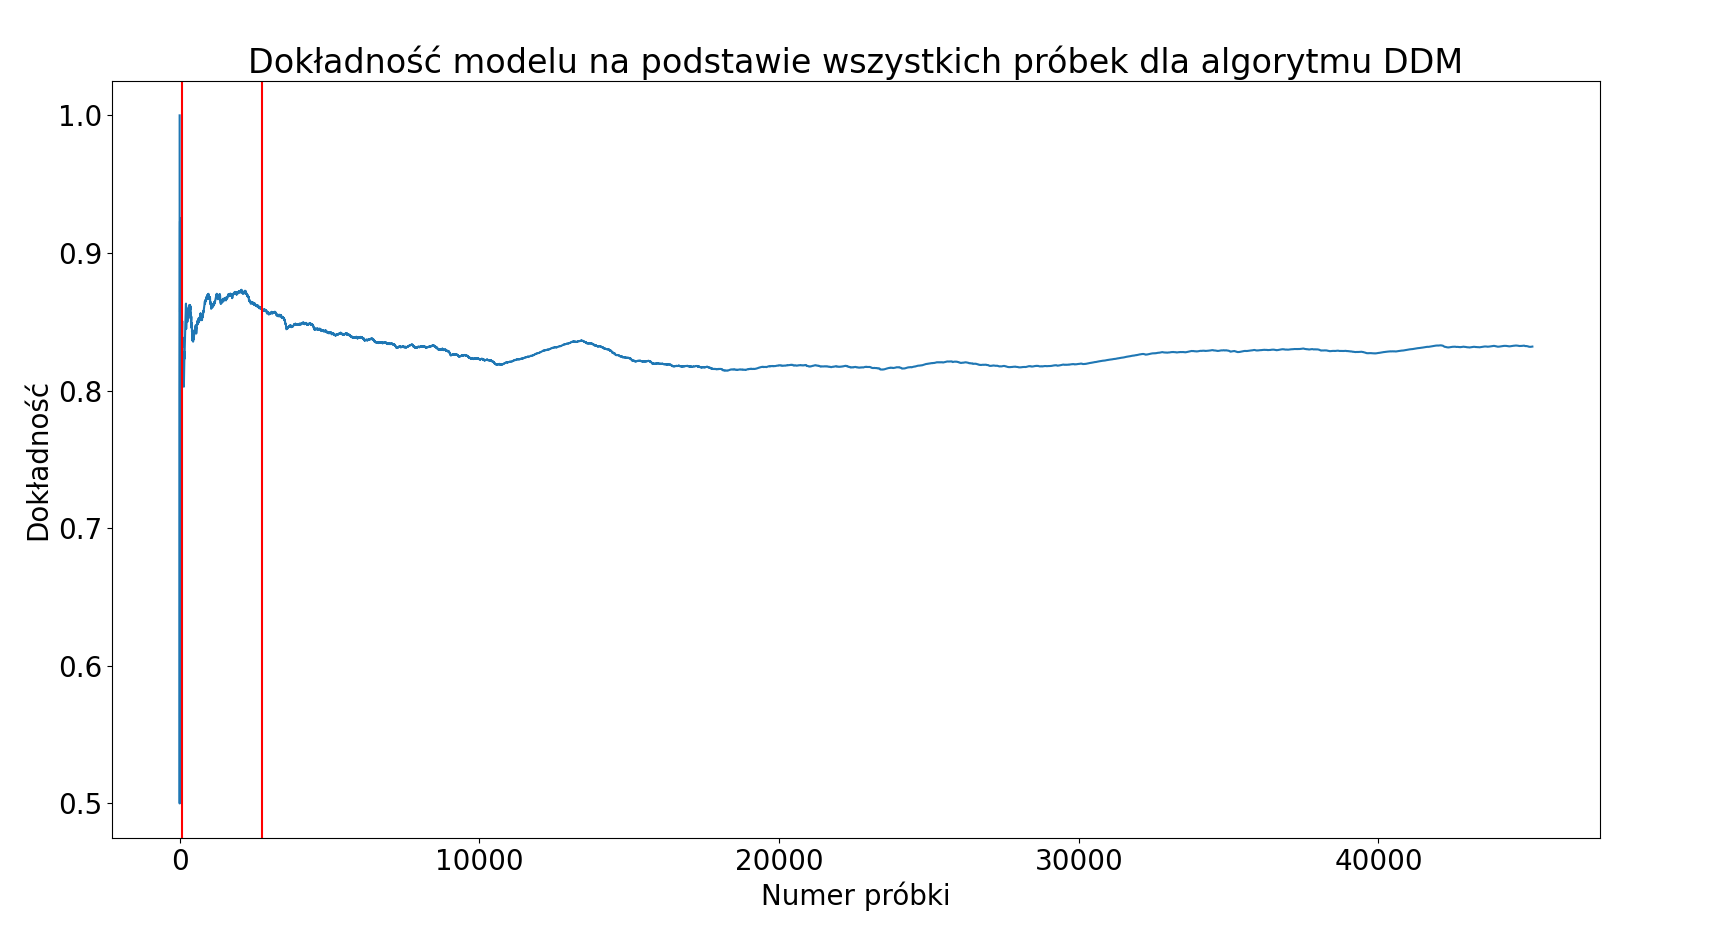
\includegraphics[width=1\textwidth]{resources/stage1/DDM.png}
%    \caption{Najczęściej zgłaszane skargi}
    \label{DDM}
\end{figure}

\begin{figure}[H]
    \centering
    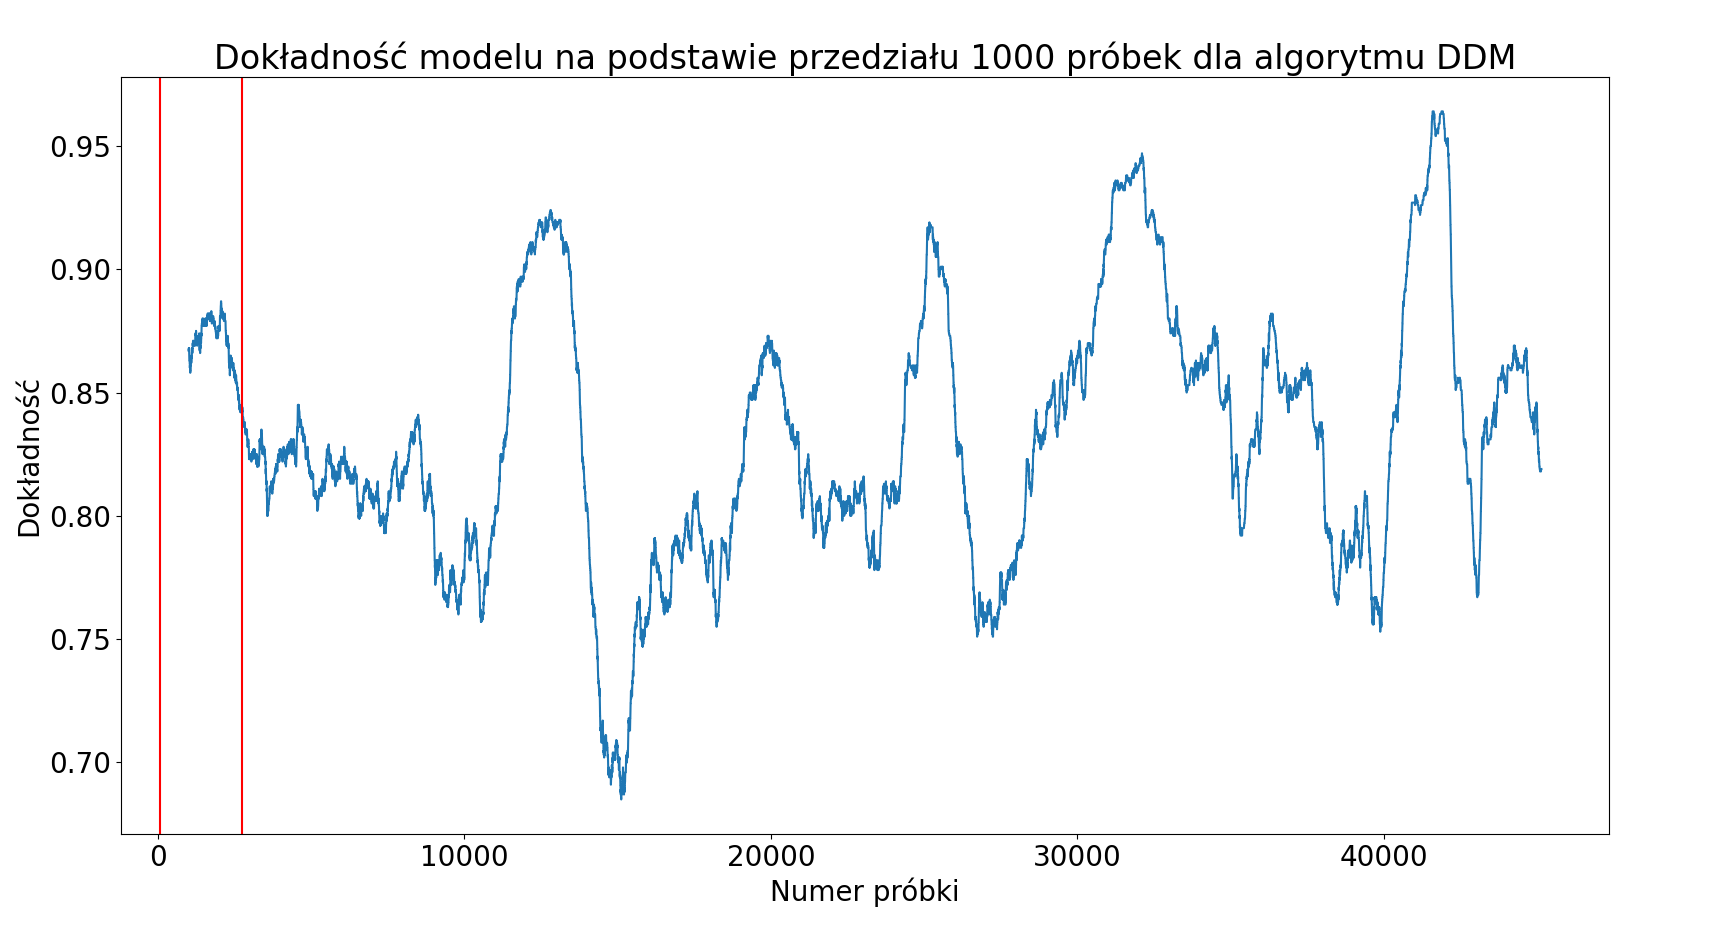
\includegraphics[width=1\textwidth]{resources/stage1/DDM_win.png}
%    \caption{Najczęściej zgłaszane skargi}
    \label{DDMw}
\end{figure}

\subsection{EDDM}

\begin{figure}[H]
    \centering
    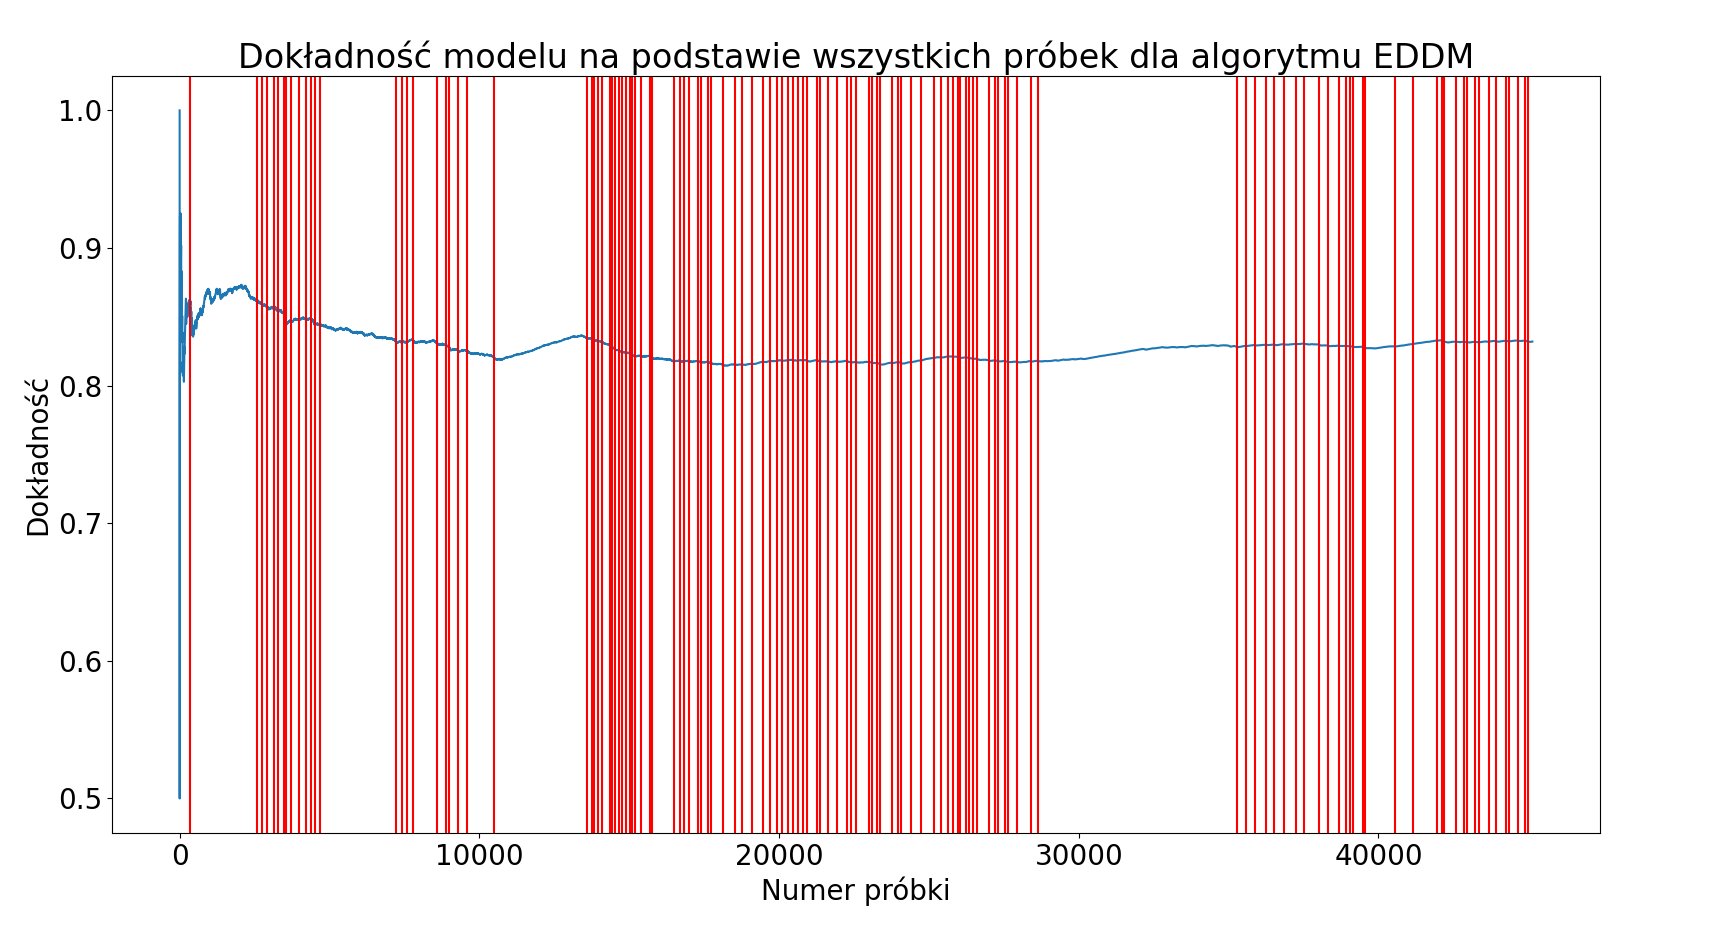
\includegraphics[width=1\textwidth]{resources/stage1/EDDM.png}
%    \caption{Najczęściej zgłaszane skargi}
    \label{DDM}
\end{figure}

\begin{figure}[H]
    \centering
    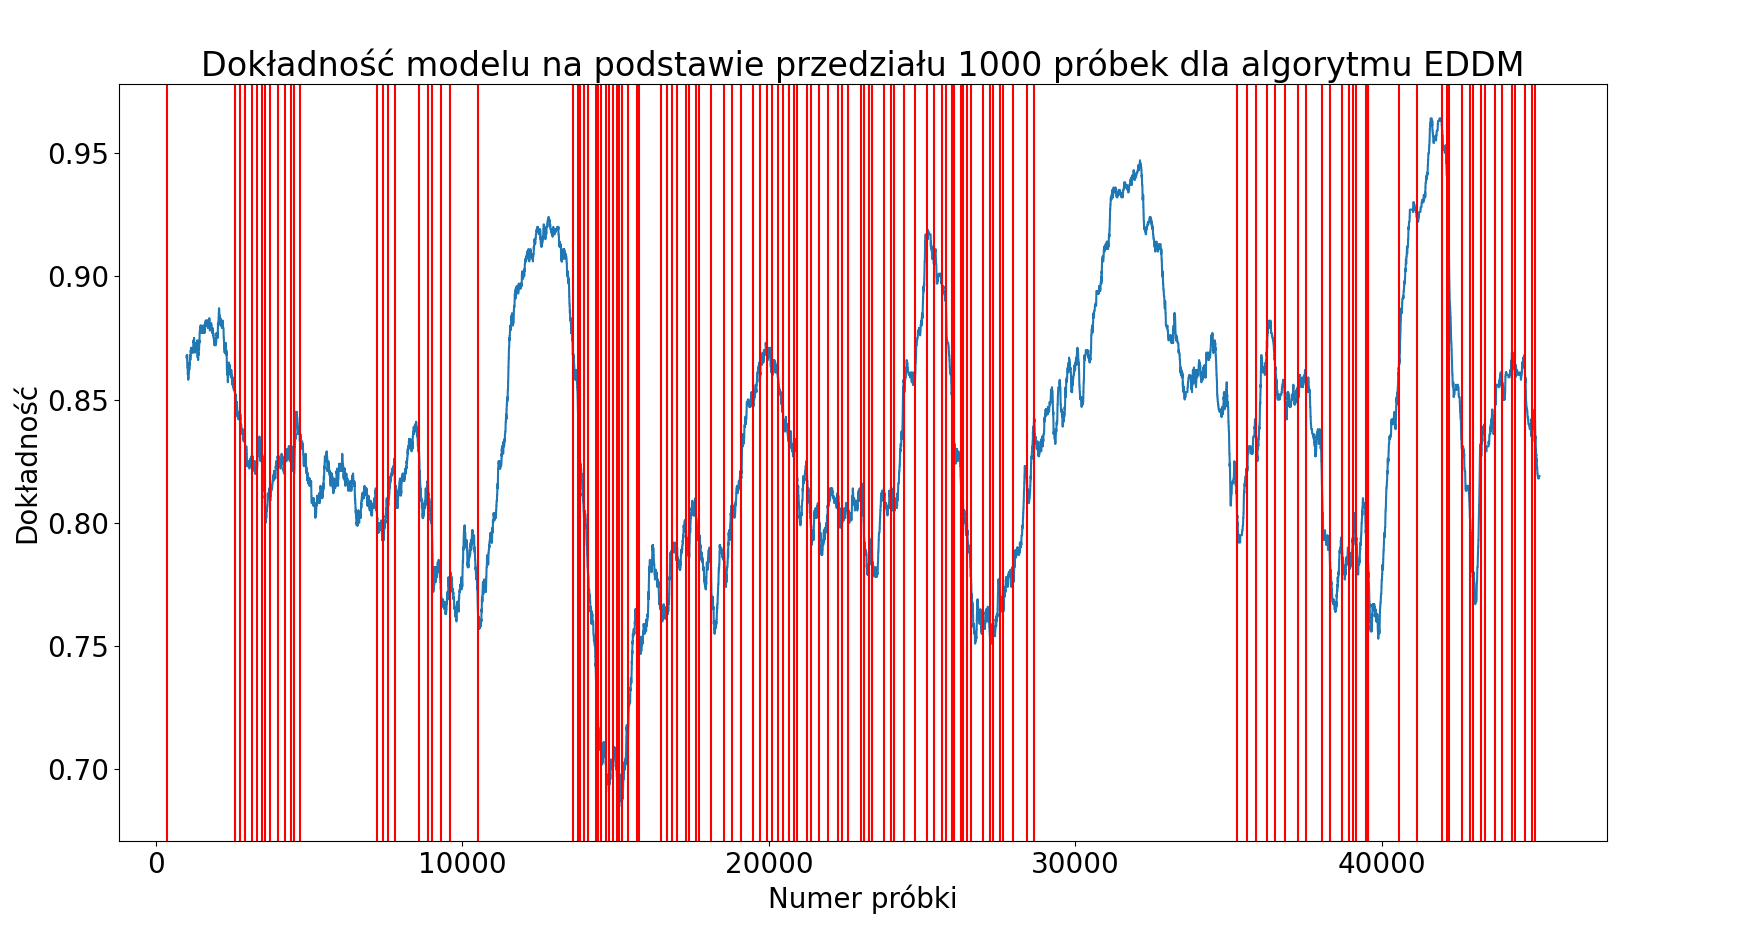
\includegraphics[width=1\textwidth]{resources/stage1/EDDM_win.png}
%    \caption{Najczęściej zgłaszane skargi}
    \label{DDMw}
\end{figure}

\subsection{ADWIN}

\begin{figure}[H]
    \centering
    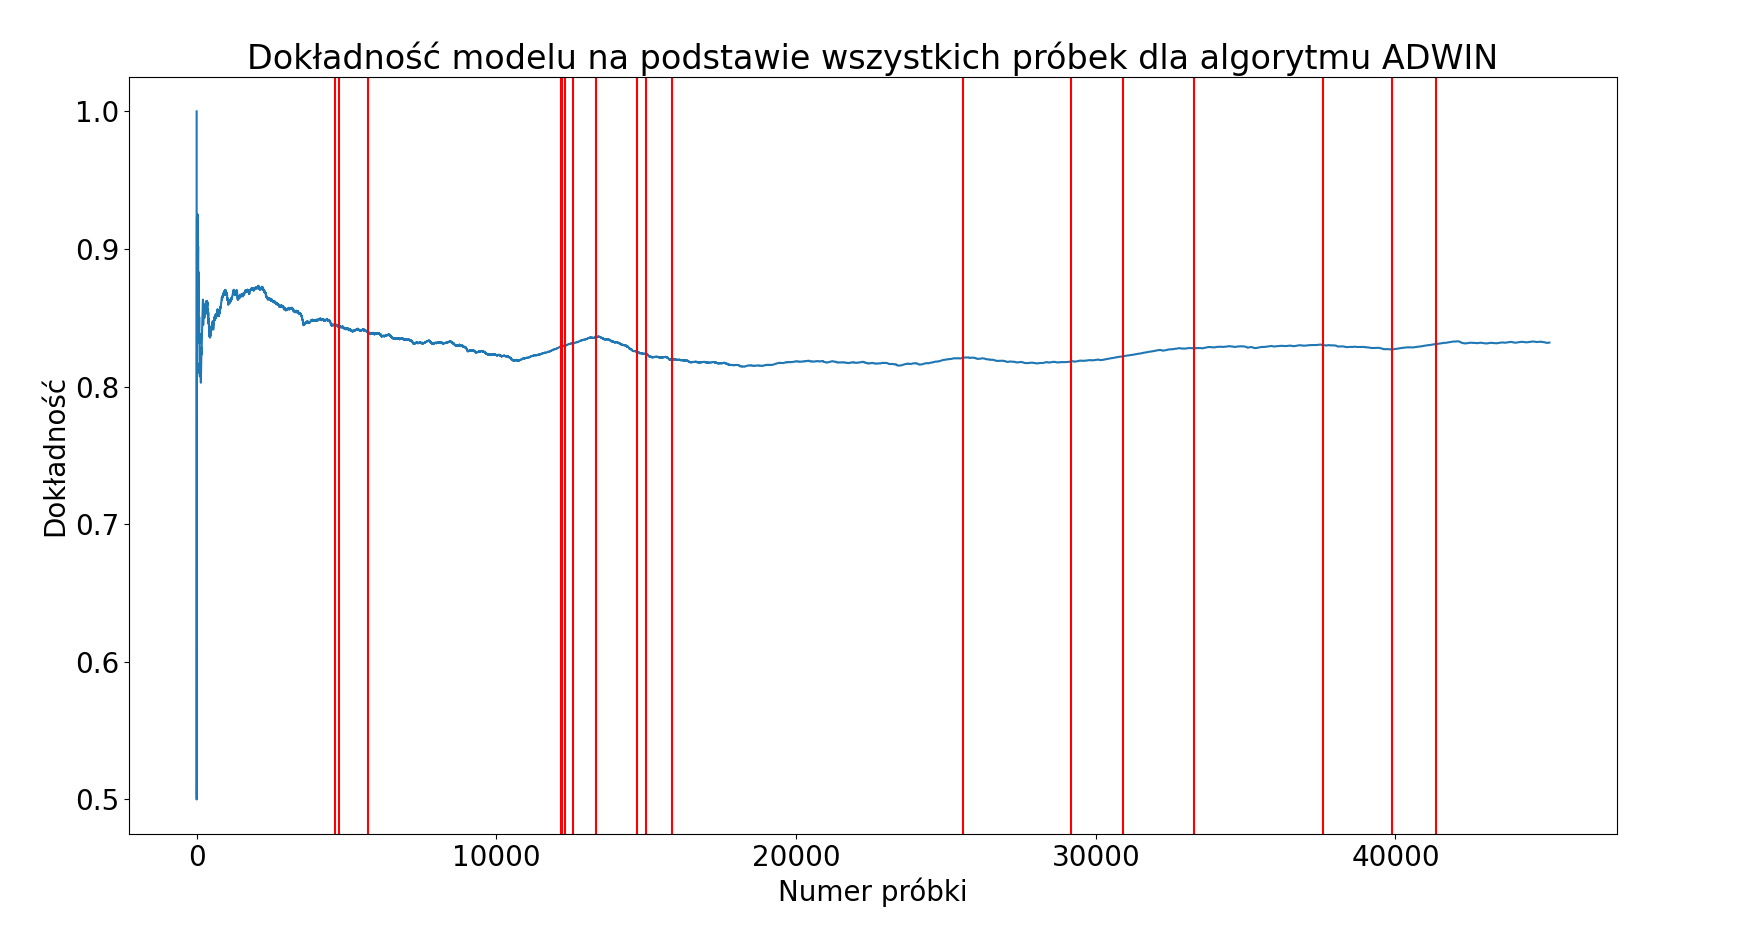
\includegraphics[width=1\textwidth]{resources/stage1/ADWIN.png}
%    \caption{Najczęściej zgłaszane skargi}
    \label{DDM}
\end{figure}

\begin{figure}[H]
    \centering
    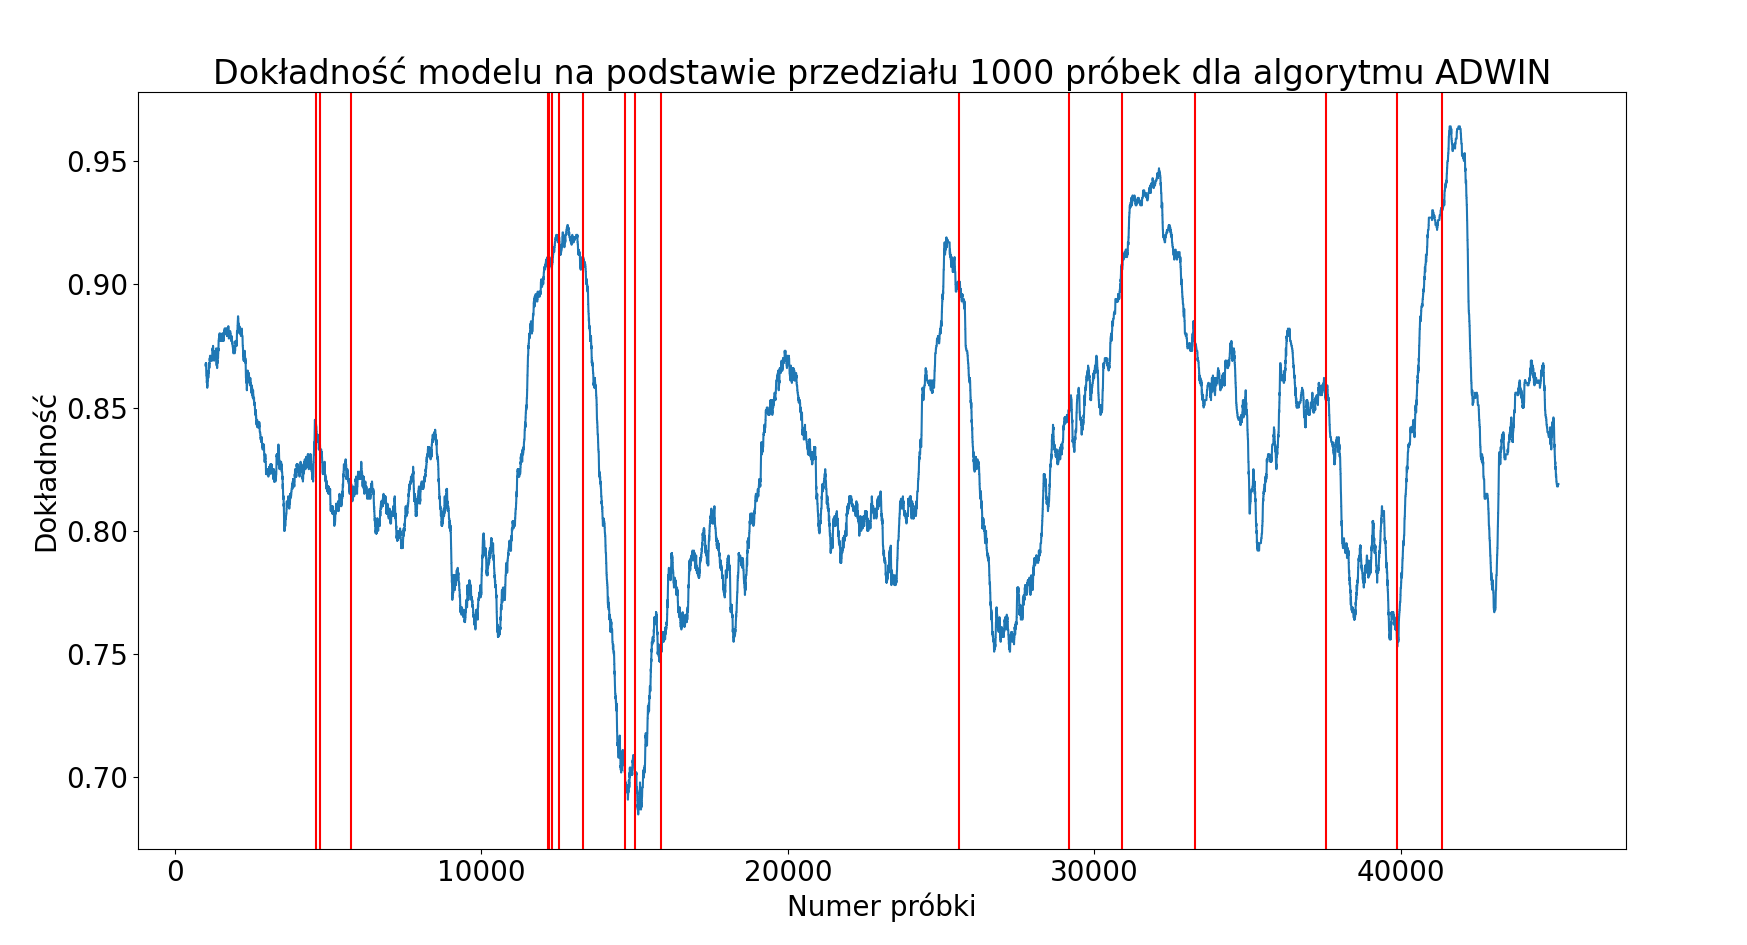
\includegraphics[width=1\textwidth]{resources/stage1/ADWIN_win.png}
%    \caption{Najczęściej zgłaszane skargi}
    \label{DDMw}
\end{figure}

\subsection{PageHinkley}

\begin{figure}[H]
    \centering
    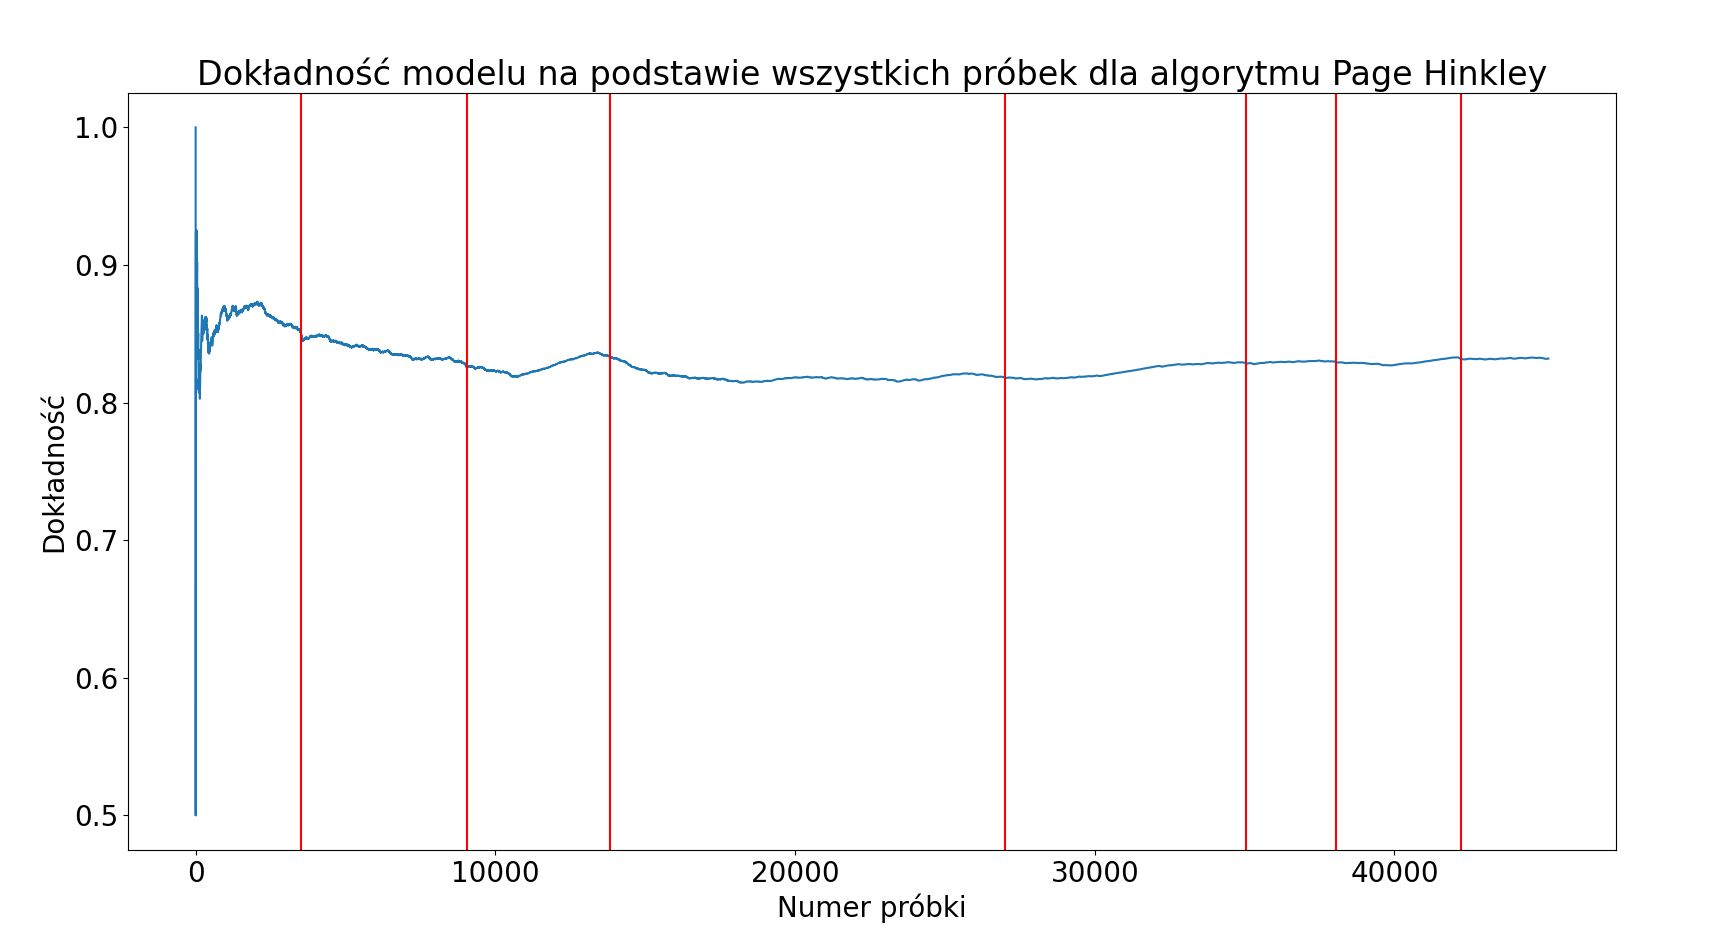
\includegraphics[width=1\textwidth]{resources/stage1/Page.png}
%    \caption{Najczęściej zgłaszane skargi}
    \label{DDM}
\end{figure}

\begin{figure}[H]
    \centering
    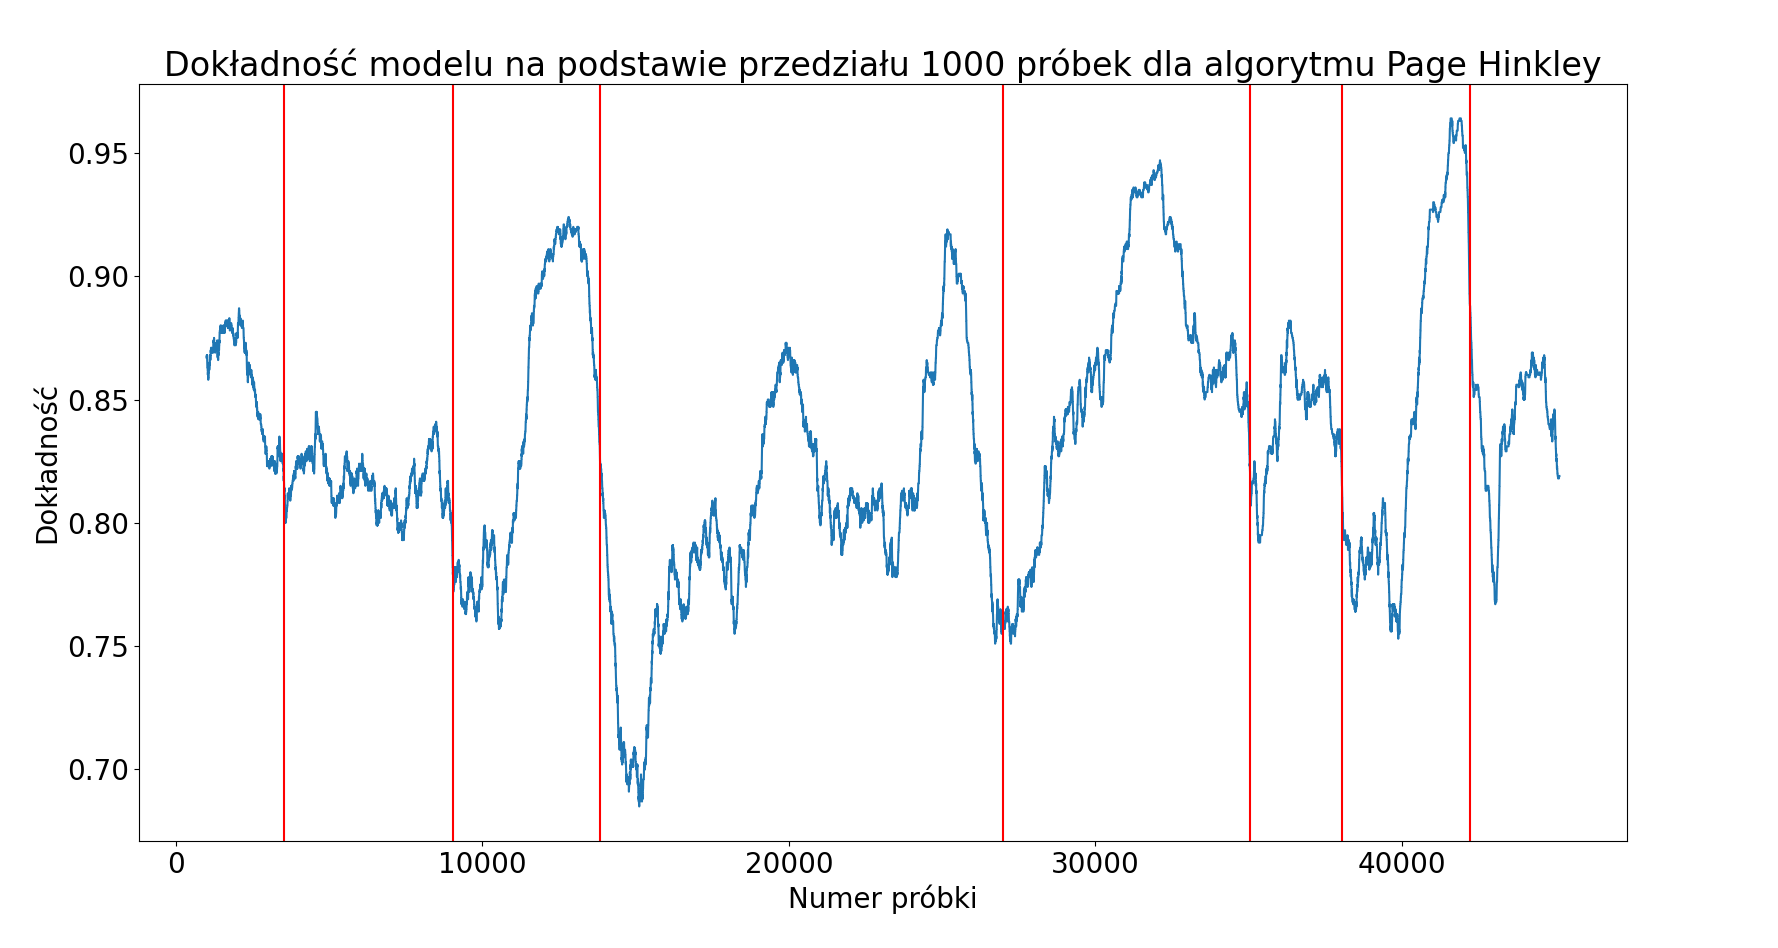
\includegraphics[width=1\textwidth]{resources/stage1/Page_win.png}
%    \caption{Najczęściej zgłaszane skargi}
    \label{DDMw}
\end{figure}

\section{Wnioski}

\begin{enumerate}
    \item Na podstawie całościowej statystyki dokładności można stwierdzić, że wybrany zbiór danych nie cechował się istotnymi zmianami modelu w czasie, dlatego też wymagane było obliczanie dokładności na podstawie n ostatnich próbek. Dzięki temu można było obliczyć aktualną dokładność modelu dla zasymulowanego przedziału czasowego.
    \item W związku z brakiem nagłych zmian modelu w zbiorze danych, algorytm DDM nie był w stanie sobie dobrze poradzić. Skoki wykryte były na początku zestawu danych, co związane może być samym sposobem wyliczania statystyk. 
    \item Z drugiej strony EDDM okazał się być zbyt czuły na fluktuacje wybranego strumienia danych.
\end{enumerate}

\newpage
\nocite{*}
\begin{thebibliography}{}

    \bibitem{AdwinFlora}
    \textsl{A Survey on Classification of Concept Drift with Stream
Data, }
    \author{Shweta Kadam,}
    \url{ https://hal.archives-ouvertes.fr/hal-02062610/file/A_survey_on_classification_of_concept_drift_with_stream_data.pdf}
    \text{ [dostęp: 15.11.2020]}
    
    \bibitem{Adwin}
    \textsl{Scalable Detection of Concept Drifts on Data Streams
with Parallel Adaptive Windowing, }
    \author{Philipp M. Grulich, René Saitenmacher, Jonas Traub, Sebastian Breß, Tilmann Rabl, Volker Markl,}
    \href{https://grulich.me/assets/publications/grulich-Scalable-Detection-of-Concept-Drifts-on-Data-Streams-with-Parallel-Adaptive-Windowing.pdf}{ \verb|https://grulich.me/assets/publications/grulich-Scalable-Detection- of-Concept-Drifts-on-Data-Streams-with-Parallel-Adaptive - Windowing.pdf}
    \text{ [dostęp: 15.11.2020]}
    
    \bibitem{Page}
    \textsl{Test of Page-Hinckley, an approach for fault detection in an agro-alimentary production system}
    \author{Mouss, Hayet and Mouss, M.Djamel and Mouss, Kinza and Linda, Sefouhi}
    \url{https://www.researchgate.net/publication/4142016_Test_of_Page-Hinckley_an_approach_for_fault_detection_in_an_agro-alimentary_production_system}
    \text{ [dostęp: 15.11.2020]}
\end{thebibliography}

\end{document}
